\documentclass[a4,10pt]{article}

\usepackage{graphicx}
\usepackage{epstopdf}
\usepackage{times}
\usepackage{rotating}


\begin{document}

\begin{sidewaystable}[p]
\tiny{\begin{tabular}{|c|c|c|c|c|c|c|c|c|c|c|c|c|c|c|}
 & >p/k & <p/k & >k/100 & <k/100 & k/100 & p/k & <k & most & >k & few & k & the & some & all\\
\hline
brown. & 38 & 22 & 2 & 18 & 8 & 688 & 490 & 1532 & 1122 & 3451 & 16455 & 63376 & 81693 & 202587\\
trec.t & 0 & 0 & 0 & 0 & 0 & 0 & 0 & 0 & 0 & 0 & 18 & 460 & 222 & 192\\
geo.te & 0 & 0 & 0 & 0 & 0 & 3 & 0 & 4 & 2 & 6 & 27 & 402 & 660 & 378\\
cli-qu & 0 & 0 & 0 & 0 & 0 & 14 & 30 & 44 & 30 & 132 & 912 & 10112 & 20780 & 11312\\
wacky. & 176 & 142 & 8 & 12 & 2 & 777 & 806 & 992 & 1712 & 1358 & 3497 & 2782 & 11944 & 29148\\
\hline
total & 214 & 164 & 10 & 30 & 10 & 1482 & 1326 & 2572 & 2866 & 4947 & 20909 & 77132 & 115299 & 243617
\end{tabular}}
\end{sidewaystable}



\vspace{0.2cm}

\begin{center}
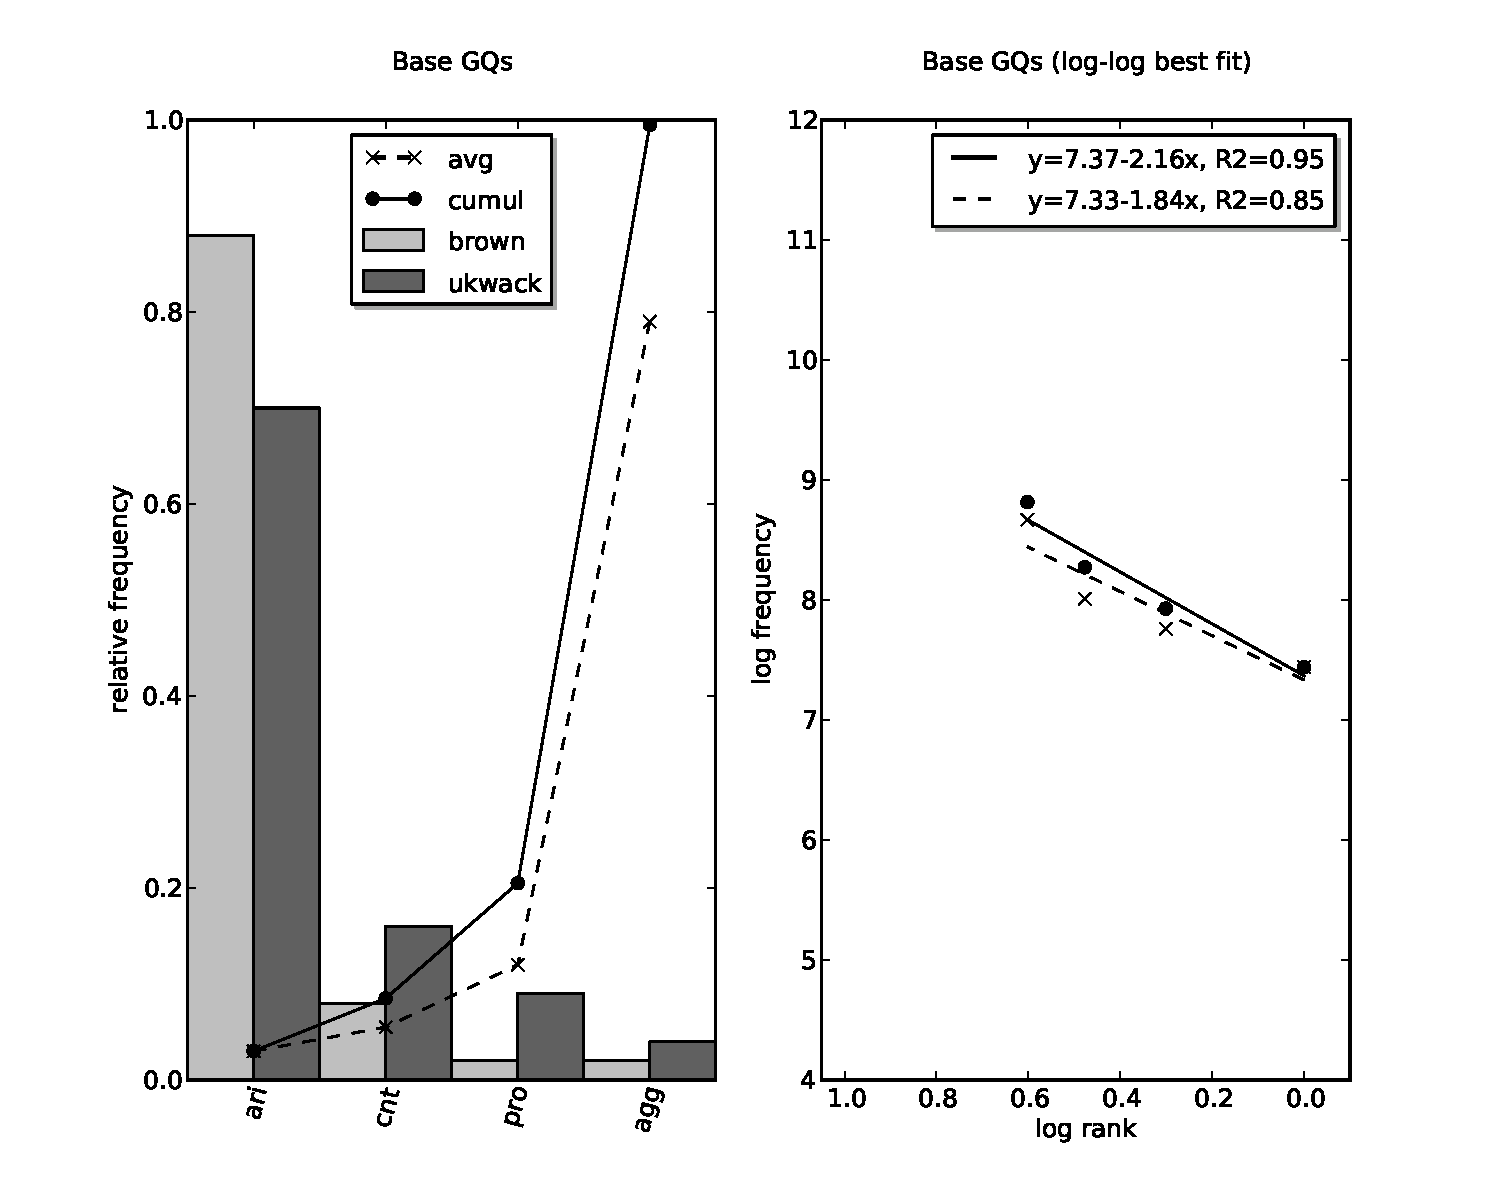
\includegraphics[scale=0.5]{/home/professors/cathorne/Desktop/quantifiers/wacky-script/plotting-par/Base-GQs-stats.pdf}
\end{center}

\end{document}